\chapter{INTRODUCCI\'ON}
\thispagestyle{empty}

El título del proyecto no debe exceder los 120 caracteres.
El título debe llamar la atención e interés sobre el trabajo desarrollado. Debe ser conciso, pertinente con la información que se presenta, exacto en el uso de términos técnicos, emplear el menor número de palabras posible y evitar la utilización de siglas, acrónimos y cualquier otra expresión redundante que pueda restarle rigor. 

Un título puede ser:
\begin{itemize}
    \item Una frase
    \item Una oración corta 
    \item Una pregunta 
\end{itemize}

\section{Texto del documento}
\textbf{Tamaño de papel:} El cuerpo del documento deberá ser elaborado en formato A4 (21 x 29,7 cm) impreso a una o doble cara.

\textbf{Márgenes de página:} 3.0 cm del margen superior, 2.0 cm del inferior, 2.5 cm izquierdo y 2.0 cm derecho.

\paragraph{Párrafo:}
Alineación justificada, espaciado 0, interlineado múltiple en 1.5.

\subparagraph{Interlineado:}
1.5 para todo el documento.

\subsection{Tablas \& Figuras}
\textbf{Tipo y tamaño de texto:}

Título: Arial 11 (negrilla, centrada), tipo oración. El primer número representa el número del capítulo y el segundo número indica el número de la tabla.
Texto tablas: Arial 10, centrada
Pie de Tabla: Arial 9. (Justificada centrada) 


\subsubsection{Tablas}
Modelo de Tablas, para referencia la tabla se usa el (label) y se lo llama asi: Tabla \ref{tbl:modelo}, la referencia y el label sirven para hacer la referencia cruzada con el indice de tablas
% Si desea crear tablas puede utlizar la herramienta https://www.tablesgenerator.com/#
% COnsiderando siempre que debe llevar la configuracion [!htbp] y centrada

\begin{table}[!htbp]
\centering
\small
\caption{{\fontsize{11pt}{13}\selectfont \textbf{Modelo General de las Tablas \cite{upm56279}}}}
\label{tbl:modelo}
\begin{tabular}{@{}cccc@{}}
\toprule
\textbf{Columna 1} & \textbf{Columna 2} & \textbf{Columna 3} & \textbf{Columna 4} \\ \midrule
Texto              & Texto              & Texto              & Texto              \\
Texto              & Texto              & Texto              & Texto              \\
Texto              & Texto              & Texto              & Texto              \\ \bottomrule
\end{tabular}
\end{table}

\subsubsection{Figuras/Gráficos:}
Modelo de las Figuras, para referenciar las figuras se usa el (label) y se lo llama así: Fig. \ref{fig:figura1a}, la referencia y el label sirven para hacer la referencia cruzada con el indice de las figuras

\textbf{Para cambiar el tamaño de las figuras use la etiqueta [width=0.6] cambiándole el n\'umero.}

\begin{figure}[!htbp]
    \centering
    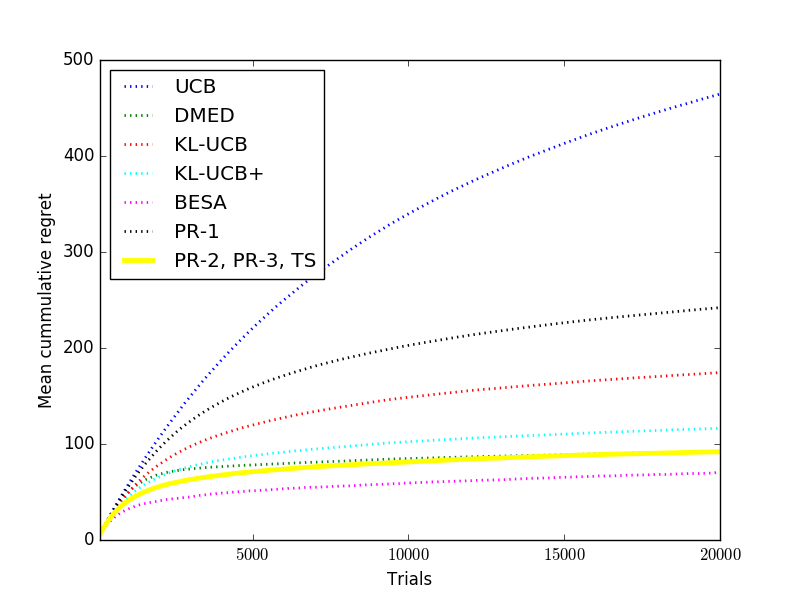
\includegraphics[width=1.0\linewidth]{recursos/Figure1a.png}
    \caption{\textbf{Modelo de las Figuras}}
    \label{fig:figura1a}
\end{figure}

Si queremos seguir agregando figuras solo copiar el código de figuras y tener siempre la etiqueta centering y [!htbp]

\begin{figure}[!htbp]
    \centering
    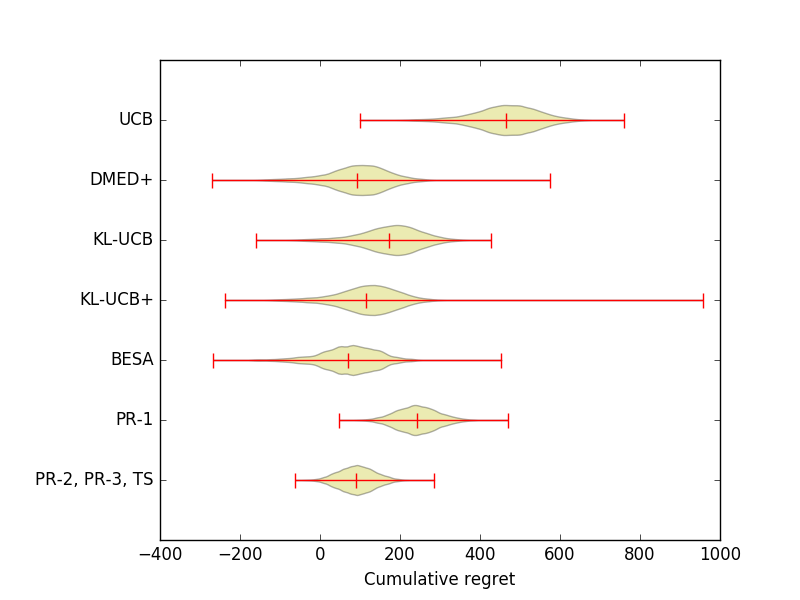
\includegraphics[width=0.85\linewidth]{recursos/Figure1b.png}
    \caption{\textbf{Modelo de las Figuras 1b \cite{upm56279}}}
    \label{fig:figura1a}
\end{figure}

\begin{figure}[!htbp]
    \centering
    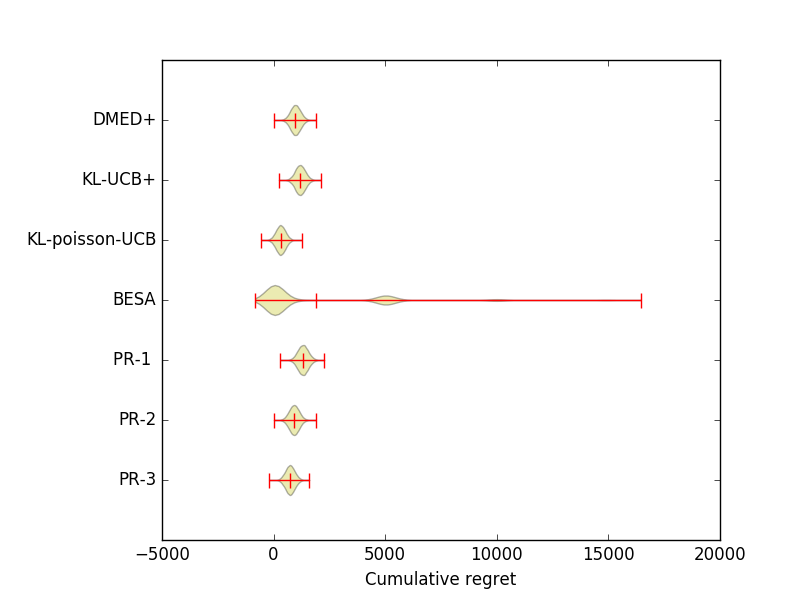
\includegraphics[width=0.85\linewidth]{recursos/Figure2.png}
    \caption{\textbf{Modelo de las Figuras 2 \cite{upm56279}}}
    \label{fig:figura1a}
\end{figure}

\section{Ecuaciones}
Si el autor utiliza ecuaciones en su documento, podrá seguir el siguiente formato: (x,z) donde x es el número del capítulo y z el número en orden de aparición de la ecuación. Como ejemplo, ver la ecuación 2.1.

\begin{equation}
\label{eqn:01}
x=kh; k = 
\begin{cases} 
0.565  & \mbox{for } men   \\
0.550  & \mbox{for } women
\end{cases}
\end{equation}

\subsection{Inercia del cuerpo humano}

Focusing on the legs, they can be approximated as uniform bars. Thus, the inertia with respect to $O$ is given by \cite{ref:young2006sears}:

\begin{equation}
\label{eqn:02}
I_l = \frac{1}{3}m_ll^2
\end{equation}

Importante decir que para hacer las referncias en los texto se debe utilizar el (label). Luego utilizar la referencia cruzada ejemplo: Lo que se enuncia en la ecuación \ref{eqn:02}.

\textbf{Una herramienta que les podría servir es, (mirar pie de página)\footnote{https://www.codecogs.com/latex/eqneditor.php?lang=es-es}:  \'o pueden conseguir otras online. }

\section{Algoritmos}
El Algoritmo \ref{alg:getDelay} ilustra la forma que debe adoptarse. Se usa el paquete \textit{algorithmic}. Los comandos pueden consultarse en \url{https://en.wikibooks.org/wiki/LaTeX/Algorithms} o en la documentación oficial.

\begin{algorithm}[htbp]
	\begin{algorithmic}
	\REQUIRE $t_0$ = instante en el que se genera el retardo
	
	\IF{$(update\_architecture==1)$}
		\IF{$(delay\_scenario==1)$}
			\STATE{delay$=C$}
		\ELSE
			\IF{$(reward\_scenario==1)$}
				\STATE{delay $\leftarrow [0,300]$-trunc\_Exp($\lambda=1/80$)}
			\ELSE
				\STATE{delay $\leftarrow [0,480]$-trunc\_Exp($\lambda=1/150$)}
			\ENDIF
		\ENDIF
	\ELSE
		\STATE{delay = difference(24:00, $t_0$)}
	\ENDIF
	
	\RETURN delay
	\end{algorithmic}
	\caption{\textbf{Algoritmo para ver los retardos - $getDelay(t_0)$}}
	\label{alg:getDelay}
\end{algorithm}
